\chapter{认识硬件}
\section{一般台式机键盘}
如图1:1;由于此年龄的家长通常会接触到手机和台式机,首先来介绍一下台式机的常用功能键。
\section{台式机常用功能键}
\footnote{以下顺序按照键盘上由上至下由左至右的顺序,可直接对照自己键盘寻找}
\subsection{Esc(退出键)}
\begin{itemize}
	\item 退出全屏
	
	打开视频或者PPT的全屏时,若要退出全屏可直接按 Esc 键退出
	\item 退出当前开启小界面
	
	当点错某个网址,可以直接按 Esc 键退出打开当前网页
	\item 清空表格
	
	即清空当前编辑表格内的全部内容。
\end{itemize}
\begin{figure}
	\centering
	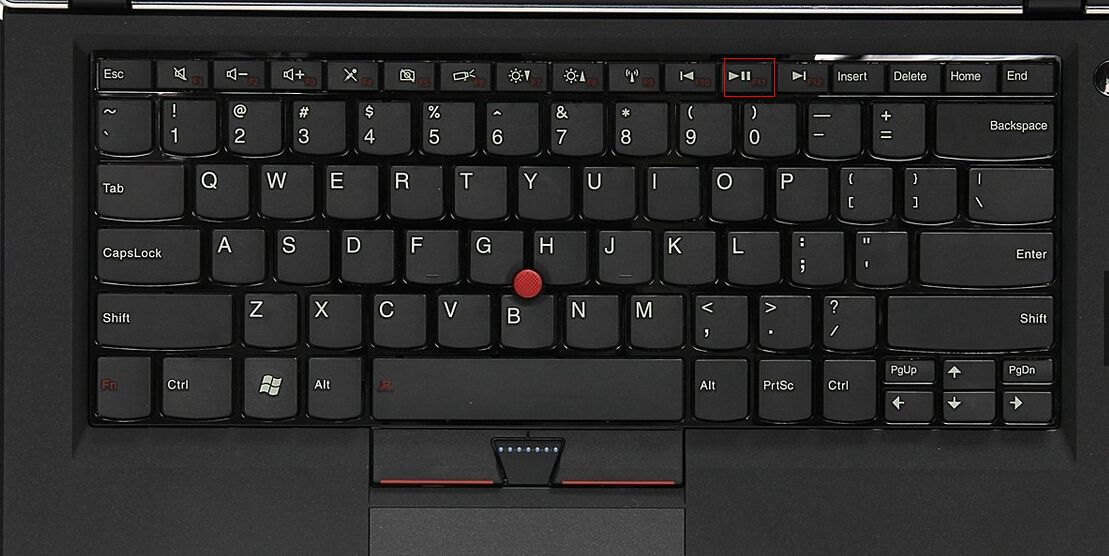
\includegraphics[width=0.7\linewidth]{../../1}
	\caption{}
	\label{fig:1}
\end{figure}
\subsection{Tab(表格键)}
\begin{itemize}
	\item 缩进字符
	
	当有很多空格需要打时,就使用 Tab 键。
\end{itemize}
\subsection{Caps(英文大小写切换)}
\subsection{Shift(切换键)}
\begin{itemize}
	\item 一般 Ctrl + Shift 键表示输入法循环并切换到所需要输入法(五笔,简体拼音,英文等)。
	\item 切换半角和全角
	\footnote{半角简单来说就是英文字符,占一个空间的一半;全角就是中文字符,占满整个空间。}
	\item Del + Shift 不经过回收站直接删除文件
	
	这种删除很难找回,建议误操作后找专人来清,当时不要选择重启或载入文件。
	\item {取消开机时启动其他附属软件}
	
	在开机界面出来后长按 Shift 键,可以避免电脑隐藏软件的开机自启动。一般电脑里不经意安装的游戏或者附属软件,可以避免恶意开启占用网速。
\end{itemize}
\subsection{Ctrl(控制键)}
不长篇赘述,之后会讲到组合键系列。
\subsection{Win(菜单键)}
\begin{itemize}
	\item 打开开始菜单
	\item 配合字母“E”打开文件夹:Win+E
	\item 配合字母“D”最小化所有窗口:Win+D
\end{itemize}
\subsection{Alt(替换键)}
不长篇赘述,之后会讲到组合键系列
\subsection{Enter(回车键)}
\begin{itemize}
	\item 换行
	\item 确认当前所打内容
\end{itemize}